% Propósito: mostrar que la cadena auditiva pasiva transfiere y transforma
% energía, mientras parte puede almacenarse, salir de la vía o disiparse, sin
% creación de energía.
% Origen: balance E_entrada=Delta E_mec+E_salida+E_disipada, ecuación
% \eqref{eq:u2-balance-energia}, aplicado cualitativamente a la relación con
% Fonoaudiología. No representa eficiencias ni datos anatómicos.
% Descripción accesible: la energía mecánica de una perturbación en el aire
% llega a la membrana timpánica, pasa a la cadena osicular y se transfiere hacia
% el oído interno. Desde la membrana y la cadena salen flechas hacia una caja de
% energía interna u otras vías, que representan almacenamiento, transferencia
% fuera de la vía principal y disipación. Ninguna etapa crea energía.
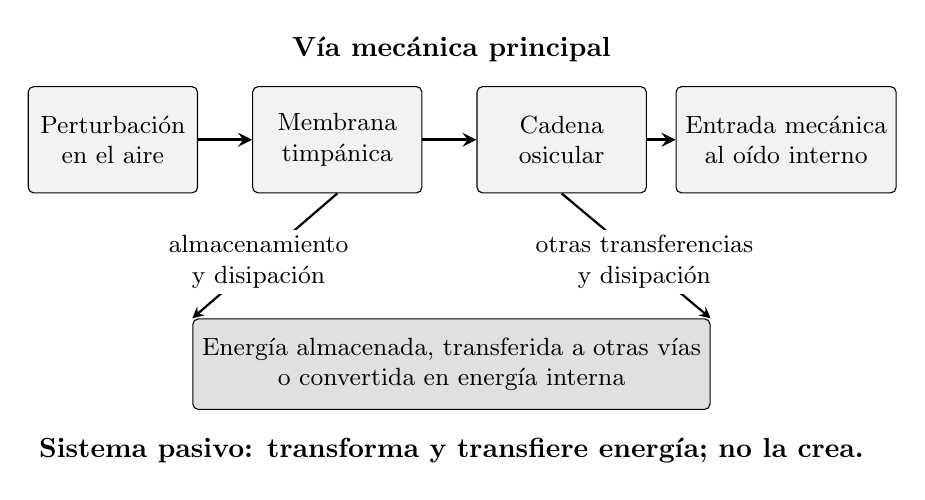
\begin{tikzpicture}[
    font=\small,
    >=stealth,
    bloque/.style={
        draw,
        rounded corners=2pt,
        minimum width=2.15cm,
        minimum height=1.35cm,
        align=center,
        fill=black!5
    }
]
    \node[bloque] (aire) at (0,0)
        {Perturbación\\en el aire};
    \node[bloque] (membrana) at (2.85,0)
        {Membrana\\timpánica};
    \node[bloque] (osiculos) at (5.7,0)
        {Cadena\\osicular};
    \node[bloque] (salida) at (8.55,0)
        {Entrada mecánica\\al oído interno};

    \node[font=\bfseries] at (4.3,1.15) {Vía mecánica principal};
    \draw[->,very thick] (aire.east) -- (membrana.west);
    \draw[->,very thick] (membrana.east) -- (osiculos.west);
    \draw[->,very thick] (osiculos.east) -- (salida.west);

    \node[
        draw,
        rounded corners=2pt,
        minimum width=5.8cm,
        minimum height=1.15cm,
        align=center,
        fill=black!12
    ] (otras) at (4.3,-2.85)
        {Energía almacenada, transferida a otras vías\\
        o convertida en energía interna};

    \draw[->,thick] (membrana.south) -- (otras.north west);
    \draw[->,thick] (osiculos.south) -- (otras.north east);
    \node[fill=white,align=center,inner sep=2pt] at (1.85,-1.55)
        {almacenamiento\\y disipación};
    \node[fill=white,align=center,inner sep=2pt] at (6.75,-1.55)
        {otras transferencias\\y disipación};

    \node[font=\bfseries] at (4.3,-3.95)
        {Sistema pasivo: transforma y transfiere energía; no la crea.};
\end{tikzpicture}
